\documentclass[a4paper,12pt,titlepage]{scrartcl}
\usepackage[sc]{mathpazo} % Schrift - wie Funcky und in PDF zu Fonts beschrieben
\usepackage[T1]{fontenc}
\usepackage[utf8]{inputenc}
\usepackage[a-1b]{pdfx}
\usepackage[ngerman]{babel}
\usepackage[amssymb]{SIunits} 
\usepackage{graphicx} 
\usepackage{subfigure}                         
\usepackage{float}
\usepackage[iso,german]{isodate} %his package provides commands to switch between different date formats
\usepackage{hyperref}
\usepackage{listings}

\usepackage{fancyhdr}
\renewcommand{\headrulewidth}{0.5pt}
\renewcommand{\footrulewidth}{0.5pt}
%Abstand zwischen Absätzen, Zeilenabstände
\voffset26pt 
\parskip6pt
%\parindent1cm  %Rückt erste Zeile eines neuen Absatzes ein
\usepackage{setspace}
\onehalfspacing

\begin{document}
\pagenumbering{roman}
\titlehead
{
    \small
    {
        Technische Universität Ilmenau\\
        Fakulät IA\\
        Fachgebiet Schaltsysteme\\

        Praktikum Schaltsysteme\\
        WS 2021/22}
}

\title {Versuchsprotokoll}
\subtitle{Versuche A3 und A10}
\author{}
\date{04.11.2021\\*[60pt]}
\maketitle

\pagestyle{fancy}
\fancyhead[R]{Praktikumsbericht: Schaltsysteme}
\pagenumbering{arabic}
\newpage

\section*{Aufgabe 2: Rechts/Links-Impulserzeugung}
Entwerfen Sie einen Automaten zur Ermittlung der relativen x-Position einer PC-Maus.
Das Maus-Modul generiert die Signale $x_0$ und $x_1$ entsprechend der folgenden Kurvenverläufe.
Durch den Automaten sind entsprechend dem angegebenen Impulsschema die Signale $l$ und $r$ zu generieren, die zur Anzeige der relativen Position an einen Vor-/Rückwärtszähler angeschlossen werden sollen.

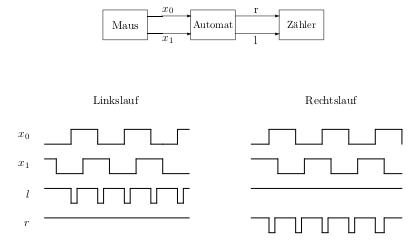
\includegraphics{Assets/Schaltsysteme-praktika-v2.png}

\section*{Aufgabe 3: Kreuztisch}
Gesucht ist ein Steuerwerk, welches durch Auswertung der Positionssignale $x_l,x_r,x_u,x_o$ und Erzeugung der Motorsteuersignale $y_l,y_r,y_u,y_o$ folgenden Ablauf realisiert:
\begin{itemize}
    \item Der Punkt P soll unabhängig von seiner Anfangsstellung nach der Pulldown-Flanke von x s
    möglichst schnell nach links/unten bewegt werden.
    \item Danach soll er am linken Rand nach oben
    \item und am oberen Rand nach rechts gefahren werden, worauf die Bewegung gestoppt werden soll.
\end{itemize}
Ein Neustart ist nur mit einer erneuten Pulldown-Flanke von $x_s$ möglich.

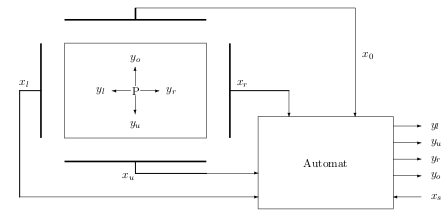
\includegraphics{Assets/Schaltsysteme-praktika-v3.png}

\section*{Aufgabe 4: Pumpensteuerung (statisch)}
Entsprechend der folgenden Skizze sollen zwei Pumpen einen Wasserbehälter füllen. Das Verhalten der Verbraucher ist nicht bekannt.
Die vier Füllstandsmelder $x_0$ bis $x_3$ sprechen jeweils bei Überschreitung eines bestimmten Füllstandes statisch an.
Die Pumpen sollen entsprechend dem angegebenen Diagramm arbeiten, wobei die Schalthäufigkeit der Pumpen gleich verteilt sein soll. Um ein ,,Flattern'' der Pumpen bei Füllständen im Bereich der jeweiligen Füllstandsmelder zu vermeiden, ist das gegebene Hystereseverhalten zu realisieren.
Entwerfen Sie eine Steuerung, die diese Aufgabe realisiert!

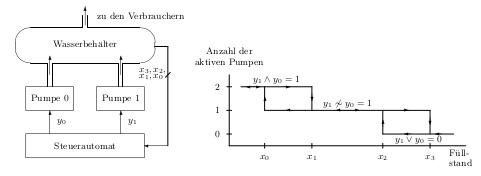
\includegraphics{Assets/Schaltsysteme-praktika-v4.png}

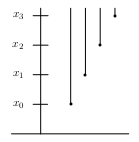
\includegraphics{Assets/Schaltsysteme-praktika-v4-2.png}
Hinweis: Bei Erreichen eines Schaltpunktes wird das Signal statisch auf 1 gesetzt. Alle Füllstandsmelder, die vom Wasser bedeckt sind, bleiben gesetzt, d.h. für den obersten Schaltpunkt ergibt sich: $x_3 x_2 x_1 x_0$.



\section*{Aufgabe 10: Ampelsteuerung}
Es soll eine Ampelsteuerung realisiert werden, die im Ruhezustand für den Autofahrer grün zeigt und auf Anforderung eines Fußgängers diesem das sichere Überqueren der Straße ermöglicht. Die dazu nötigen Phasen zeigt die folgende Tabelle.
\begin{tabular}{c|c|c|c}
    Zustand & Autoampel & Fußgängerampel & Dauer(s)\\
    S1 & grün & rot & Ruhezustand \\
    S2 & gelb & rot & 3 \\
    S3 & rot & rot & 3 \\
    S4 & rot & grün & 24 \\
    S5 & rot & rot & 12 \\
    S6 & rot-gelb & rot & 3
\end{tabular}
Die Steuerung hat eine Taktfrequenz von $\frac{1}{3}$ Hz.
Entwerfen Sie eine Steuerung, die diese Aufgabe realisiert!


\end{document}